\chapter{Programmability and Productivity}
\label{chapter:compare}

As previously mentioned, the StreamIt language aims to improve 
programmability for streaming applications. This chapter expands 
on this topic by giving specific instances from the MPEG-2 codec 
implementations where StreamIt improved programmer productivity.

Section~\ref{sec:buffer_management} focusses on StreamIt's 
implicit buffer management. Section~\ref{sec:pipelines_block}
describes how pipelines preserve the block diagram structure
in the program definition and provide a one-to-one mapping with
code. Sections~\ref{sec:expose_data}~and~\ref{section:chroma}
show StreamIt's ability to expose data distribution and
how this leads to a high degree of malleability. 
Section~\ref{sec:hier} describes the advantages of
hierarchical stream graph construction and 
Section~\ref{sec:teleport_useful} the advantages of 
teleport messaging.

Because I particularly want to contrast with 
traditional languages, a number of C code comparisons appear in 
this and the subsequent section. These code examples come from the 
C reference decoder implementation~\cite{reference-mpeg-c} provided 
by the MPEG Software Simulation Group and used in the 
MediaBench~\cite{lee97mediabench} benchmark suite. Because our 
StreamIt code does not support interlacing or certain optional 
bitstream semantics, I have modified the C reference implementation 
to remove that additional functionality, for the purposes of fair 
comparison. The comparison is between the StreamIt decoder of $2282$ 
lines, and the C reference code of $3477$ lines\footnote{As before, line counts 
were generated using \texttt{SLOCcount}~\cite{sloccount}.}. 
I believe this line count comparison is a fair 
quantization of StreamIt's ability to concisely express the MPEG-2 
decoder computations.

\section{Buffer Management}
\label{sec:buffer_management}

\begin{figure}
  \begin{center}
    \begin{minipage}{4in}
      \begin{small}
        \begin{verbatim}
01 static void Add_Block(comp,bx,by)
02      int comp,bx,by;
03 {
04   int cc,i, j, iincr;
05   unsigned char *rfp;
06   short *bp;
08   cc = (comp<4) ? 0 : (comp&1)+1;
09   if (cc==0) {
10     rfp = current_frame[0] + 
11           Coded_Picture_Width*(by+((comp&2)<<2)) + 
12           bx + 
13           ((comp&1)<<3);
14     iincr = Coded_Picture_Width - 8;
15     if (chroma_format!=CHROMA444)
16       bx >>= 1;
17     if (chroma_format==CHROMA420)
18       by >>= 1;
19     rfp = current_frame[cc] + 
20           Chroma_Width*(by+((comp&2)<<2)) + 
21           bx + 
22           (comp&8);
23     iincr = Chroma_Width - 8;
25   }
26   bp = ld->block[comp];
27   for (i=0; i<8; i++) {
28     for (j=0; j<8; j++) {
29       *rfp = *bp++ + *rfp;
30       rfp++;
31     }
32     rfp+= iincr;
33   }
34 }
        \end{verbatim}
      \end{small}
    \end{minipage}
  \end{center}
  \caption{Combining the spatially and temporally decoded data in C.}
  \label{fig:add-filter-in-c}
\end{figure}

\begin{figure}
  \begin{center}
    \begin{minipage}{3in}
      \begin{small}
        \begin{verbatim}
01 int->int filter Add_Block {
02   work pop 2 push 1 {
03     push(pop()+pop());
04   }
05 }
        \end{verbatim}
      \end{small}
    \end{minipage}
  \end{center}
  \caption{Combining the spatially and temporally decoded data in StreamIt.}
  \label{fig:add-filter2}
\end{figure}

Figure~\ref{fig:add-filter-in-c} shows the C code responsible for merging the
spatially and temporally decoded block data\footnote{The original Add\_Block function
performed some unrelated parts of the decoding process as well and was almost 99 lines
long. For comparison purposes the unrelated code is removed.}. Prior to the execution of this
function the IDCT function has generated the motion prediction
error and the motion compensation function has generated the motion prediction. 
These two sets of data are summed to produce the decoded blocks.

Lines 9 through 25 determine the appropriate memory addresses 
for the next block to be processed. Lines 26 to 33 perform the
summation.
Note that line 29 is the only line actually performing the summation. 
The buffer management details dominate every line of code and obscure its functional
purpose. 
The buffer management details are particularly complicated
because the address of the data is dependent on the block's position in a picture,
the size of the video, and the chroma format. The complicated arithmetic
used to adjust buffer indices will make it challenging for a compiler to extract
parallelism. Further complicating any compiler analysis is the function's reuse
 of an input buffer as an output buffer (as reflected in
line 29). 

Reusing buffers is one of many buffer management strategies. The strategy yielding
the best performance depends on the 
target architecture and the size of the buffer. However, the programmer has been
forced to guess about the performance and commit to a particular strategy. 
Also note that a programmer using this function must manually determine 
an execution schedule and buffer sizes that avoid buffer underflow or the premature
overwriting of data.

Now consider the equivalent StreamIt code for adding the decoded block data, shown in
Figure~\ref{fig:add-filter2}. The code itself is almost trivial. The filter 
occurs after a \texttt{roundrobin(1)} joiner merging the prediction error
and the prediction itself. Figure~\ref{fig:motion_prediction_parallel}, 
explained in detail later in Chapter~\ref{chapter:exposing_parallelism}, shows
this filter in the context of the motion compensation stream graph. Note that 
the amount of data this filter processes will 
be dependent on the same chrominance and picture size parameters as the C code
but the buffer management details are hidden from the programmer - they will
be reflected in the data rates of the splitters and joiners surrounding
the filter in the motion compensation graph. At compile
time the compiler makes the decisions about the best buffer management 
strategy~\cite{sermulins05lctes}.  

\section{Pipelines Preserve Block Structure}
\label{sec:pipelines_block}

The pipeline construct preserves the structure implicit in a block diagram.
Figure~\ref{fig:spatial_decoding1} shows a block diagram for spatial decoding
taken from Figures 7-1 and 7-4 of the MPEG-2 specification~\cite{MPEG2}.
Figure~\ref{fig:spatial_decoding0} shows the 
StreamIt code that implements the pipeline. The obvious 
correspondence points to StreamIt's ability to naturally
represent this computation. Note that the quantization
parameters in the diagram are realized as messages in the stream graph.

\begin{figure}[h]
  \center{
    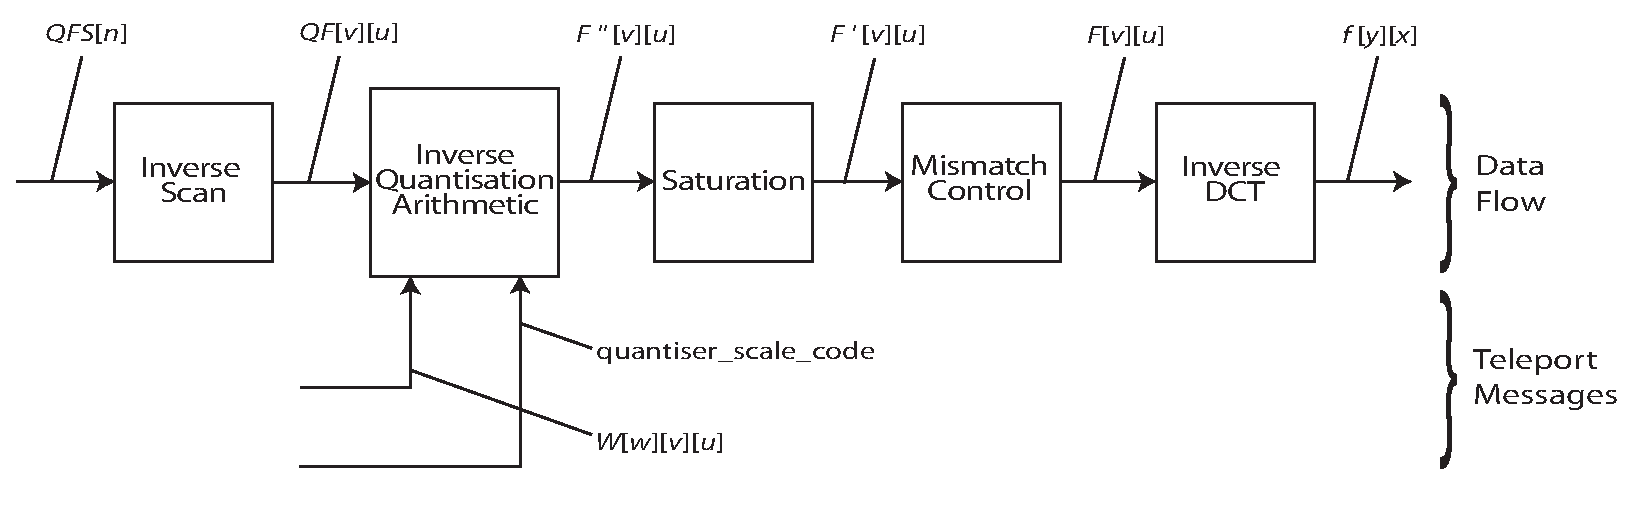
\includegraphics[scale=0.55, angle=0]{./block_decoding.eps}
    \vspace{-12pt}
 	\caption{Block diagram for spatial decoding (from MPEG-2 specification).}
 	\label{fig:spatial_decoding1}
  }
\end{figure}

\begin{figure}
  \begin{center}
    \begin{minipage}{3.5in}
      \begin{small}
        \begin{verbatim}
int->int pipeline BlockDecode(
  portal<InverseQuantization> quantiserData,
  portal<MacroblockType> macroblockType) {

  int[64] Order = {...};
  add ZigZag(64, Order);
  add InverseQuantization() to quantiserData,
                               macroblockType;
  add Saturation(-2048, 2047);
  add MismatchControl();
  add 2D_iDCT(8); // 8x8 2D IDCT
  add Saturation(-256, 255);

}
        \end{verbatim}
      \end{small}
    \end{minipage}
  \end{center}
 	\caption{StreamIt pipeline for spatial decoding.}
 	\label{fig:spatial_decoding0}
\end{figure}

An important detail to note is that each of the filters used in a pipeline
may have different granularities. In this case 
the inverse scan, quantization, and IDCT all operate on blocks of 64 data
values at a time. The mismatch control and saturation blocks are naturally expressed
in terms of a single input and output token. Nowhere must the programmer specify
the number of executions or the execution sequence needed to fully decode a picture
or video. This granularity variance holds through the rest of MPEG-2 as well.
Picture reordering can be expressed in terms of pictures and motion compensation in terms of motion vectors. 
The programmer's burden is eased since he does not have to worry about the rate discrepancies
between filters. 

\section{Natural Exposure of Data Distribution}
\label{sec:expose_data}

\begin{figure}
  \begin{center}
    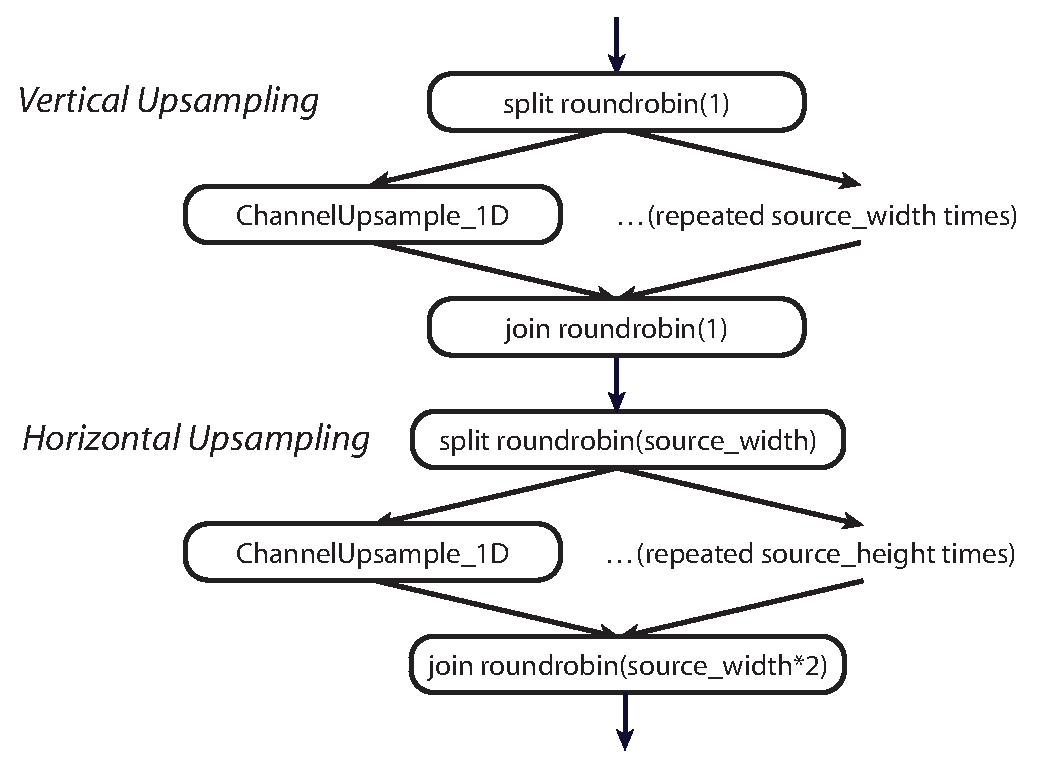
\includegraphics[scale=0.6, angle=0]{./channel_upsampling.eps}
    \caption{2D upsampling decomposed into 1D upsampling}
    \label{fig:how-upsampler-splits-data}
  \end{center}
\end{figure}

\begin{figure}
  \begin{center}
    \begin{minipage}{5.2in}
      \begin{small}
        \begin{verbatim}
int->int splitjoin ChannelUpsample_Vertical(int sourcewidth, 
                                            int sourceheight) {
    split roundrobin(1);
    for (int i = 0; i < sourcewidth; i++) {
        add ChannelUpsample_1D(sourceheight, 0.75, 0.25);
    }
    join roundrobin(1);
}

int->int splitjoin ChannelUpsample_Horizontal(int sourcewidth, 
                                              int sourceheight) {
    split roundrobin(sourcewidth);
    for (int i = 0; i < sourceheight; i++) {
        add ChannelUpsample_1D(sourcewidth, 0.5, 0.5);
    }
    join roundrobin(sourcewidth*2);
}
        \end{verbatim}
      \end{small}
    \end{minipage}
  \end{center}
  \caption{Splitjoins for channel upsampling.}
  \label{fig:upsamplecode}
\end{figure}

The splitjoin construct is a robust mechanism for expressing 
parallelism and data reordering operations. It can be used 
to specify coarse grained parallelism at the highest levels 
of an application because it exposes the independence of computational 
blocks. But it is also useful for describing how a 
computation should be performed, exposing 
coarse grained and fine grained parallelism 
as a byproduct. 

Channel upsampling illustrates this. One can easily 
think of 2D upsampling in terms of 1D upsampling in the vertical 
and horizontal direction\footnote{This is conceptually similar
to the decomposition of a 2D DCT, discussed 
later in Section~\ref{sec:2d_dct}. 
In this case the channel upsampling represents a smaller
amount of work and the splitjoin is more interesting for its
ability to efficiently express the transformation than its ability
to expose parallelism.}. The 
natural way to express upsampling a picture in either 
direction is as a parallel computation on every row or 
column of the picture. The building block is a one-dimensional 
upsampling filter that takes in a pair of weights used for 
interpolation between points. The weights are different for 
horizontal and vertical upsampling because MPEG-2 downsamples 
horizontally by removing pixels, and vertically by displacing 
them. 
The vertical upsampler splits the 
data by column and the horizontal upsampler splits the data 
by row. Figure~\ref{fig:how-upsampler-splits-data} illustrates 
the procedure and Figure~\ref{fig:upsamplecode} shows the 
StreamIt code that implements the process. The C reference
implementation implements upsampling as a series of loops
wrapped around a one dimensional upsampling kernel. In this
case the code looks similar to the StreamIt code. However,
the StreamIt \texttt{for} loops represent graph topology
resolved at initialization time. The C compiler must analyze
the body of the loops to extract parallelism.

\section{Code Malleability}
\label{section:chroma}

\begin{figure}
\begin{center}
  \begin{minipage}[t]{4.8in}
    \begin{small}
      \begin{verbatim}
   /* Y */
01 form_component_prediction(src[0]+(sfield?lx2>>1:0),
02                           dst[0]+(dfield?lx2>>1:0),
03                           lx,lx2,w,h,x,y,dx,dy,average_flag);
04 if (chroma_format!=CHROMA444)  {
05    lx>>=1; lx2>>=1; w>>=1; x>>=1; dx/=2;
06 }
07 if (chroma_format==CHROMA420)  {
08   h>>=1; y>>=1; dy/=2;
09 }
   /* Cb */
10 form_component_prediction(src[1]+(sfield?lx2>>1:0),
11                           dst[1]+(dfield?lx2>>1:0),
12                           lx,lx2,w,h,x,y,dx,dy,average_flag);
   /* Cr */
13 form_component_prediction(src[2]+(sfield?lx2>>1:0),
14                           dst[2]+(dfield?lx2>>1:0),
15                           lx,lx2,w,h,x,y,dx,dy,average_flag);    
      \end{verbatim}
    \end{small}
  \end{minipage}
  \caption{C code excerpt for handling
           4:2:0 and 4:2:2 chroma formats.}
  \label{fig:chroma-format-code-C}
\end{center}
\end{figure}

\begin{figure}
\begin{center}
  \begin{minipage}[t]{3.5in}
    \begin{small}
      \begin{verbatim}
// B = amount of data per block
// V = amount of data per motion vector
add splitjoin {
  split roundrobin(4*(B+V), B+V, B+V);
  add MotionCompensation(4*(B+V)) to PT1;
  for (int i = 0; i < 2; i++) {
    add pipeline {
      add MotionCompensation(B+V) to PT1;
      add ChannelUpsample(B);
    }
  }
  join roundrobin(1, 1, 1);
}
      \end{verbatim}
    \end{small}
  \end{minipage}
  \caption{Original StreamIt code excerpt for handling
           4:2:0 chroma format only.}
  \label{fig:chroma-format-code-streamit-previous}
\end{center}
\end{figure}

\begin{figure}
\begin{center}
  \begin{minipage}[t]{3.5in}
    \begin{small}
      \begin{verbatim}
// C = blocks per chroma channel 
//     per macroblock 
// C = 1 for 4:2:0, C = 2 for 4:2:2
// B = amount of data per block
// V = amount of data per motion vector
add splitjoin {
  split roundrobin(4*(B+V), 2*C*(B+V));
  add MotionCompensation(4*(B+V)) to PT1;
  add splitjoin {
    split roundrobin(B+V, B+V);
    for (int i = 0; i < 2; i++) {
      add pipeline {
        add MotionCompensation(B+V) to PT1;
        add ChannelUpsample(C*B);
      }
    }
    join roundrobin(1, 1);
  }
  join roundrobin(1, 1, 1);
}
      \end{verbatim}
    \end{small}
  \end{minipage}

  \caption{StreamIt code excerpt for handling
           4:2:0 and 4:2:2 chroma formats.}
  \label{fig:chroma-format-code-streamit}
\end{center}
\end{figure}

\begin{figure}
  \begin{center}
    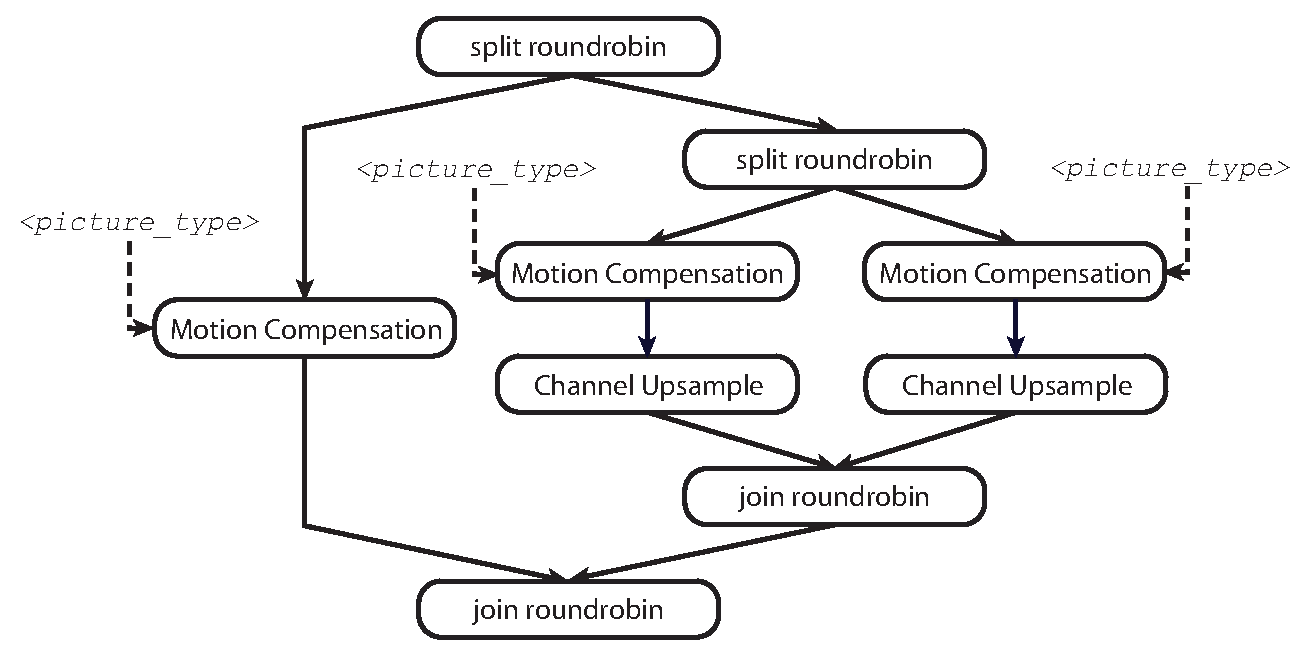
\includegraphics[scale=0.5, angle=0]{./chroma_splitjoin.eps}
    \caption{Modified subgraph for handling 4:2:0 and 4:2:2 chroma formats.}
    \label{fig:chroma-format-graph}
  \end{center}
\end{figure}

A noteworthy aspect of the StreamIt implementation is its
malleability. I illustrate this by outlining how the decoder
implementation is modified to support both 4:2:0 and 4:2:2 chroma
formats (see Section~\ref{section:picture_decomp}). 
The conceptual difference between chroma formats is merely a change in
downsampling ratio. The implementation difference is that the 4:2:0 format
represents a macroblock with six blocks, and the 4:2:2 with 8 blocks. This
change affects the data rates, and the data splitting ratios between color channels. 
In the C reference code, the change requires adjustments to buffer sizes, array lengths, array
indices, loop bounds, and various pointer offsets. The reference implementation
uses a \textbf{chroma flag} to dictate control flow and alternate
index/offset calculations in 43 locations in the code. As an example,
Figure~\ref{fig:chroma-format-code-C} shows a code fragment from the
\texttt{form\_prediction} routine in
\texttt{recon.c}. The function calls a
subroutine to perform the motion compensation on each of the three
color channels, passing in array offsets to a global array holding the
data. Lines 4-6 adjust values used for address calculations to handle
the 4:2:2 and 4:2:0 chroma formats, and lines 7-9 provide additional
adjustments for the 4:2:0 format. While these offset adjustments are
necessary in C, they are difficult for programmers and make the code
hard to understand.

In StreamIt, I modified 31 lines and added 20 new lines to support
the 4:2:2 format. Of the 31 modified lines, 23 were trivial changes to
introduce the chroma format as a stream parameter. The greatest
substantial change was to the color channel splitter, previously
illustrated on line 17 of Figure~\ref{fig:dec-with-code}. In the case
of a 4:2:2 sampling rate, the chrominance data, as it appears on the
input tape, alternates between each of the two chrominance
channels, as previously shown in Figure~\ref{fig:chroma_format}.
Thus, a nested splitjoin is used to properly recover the
chrominance channels. 

The code for the old splitjoin before the chroma format
support modifications is shown in 
Figure~\ref{fig:chroma-format-code-streamit-previous}.
The code for the new splitjoin is shown in 
Figure~\ref{fig:chroma-format-code-streamit} and
illustrated in Figure~\ref{fig:chroma-format-graph}.  
In the StreamIt code, the chroma
format explicitly dictates control flow in only 9 locations. Of
course, chroma format changes have effects on scheduling 
and buffer management, but this is transparent to the programmer.

\section{Hierarchical Construction vs Functional Calls}
\label{sec:hier}

Preserving the block structure in the program definition is important for
programmer productivity and maintaining code malleability. 
Figure~\ref{fig:call-diagram}
shows what happens to the block diagram in a traditional language. This figure
represents a simplified call trace for the MPEG-2 decoder in C. 
Note that each component must be wrapped in loops determining the exact number 
of iterations the component must run to fully decode a picture or video. 
Data is stored in global buffers and addresses to these buffers are passed between
functions, so the code structure fails to reflect the actual movement of data.
Finally, notice that the functions for parsing, motion compensation, and spatial decoding are
intermixed in the code for performance reasons.
The StreamIt compiler can interleave the phases of execution to provide performance
but this does not require the programmer to mix functional code.

\begin{figure}[h]
  \begin{center}
    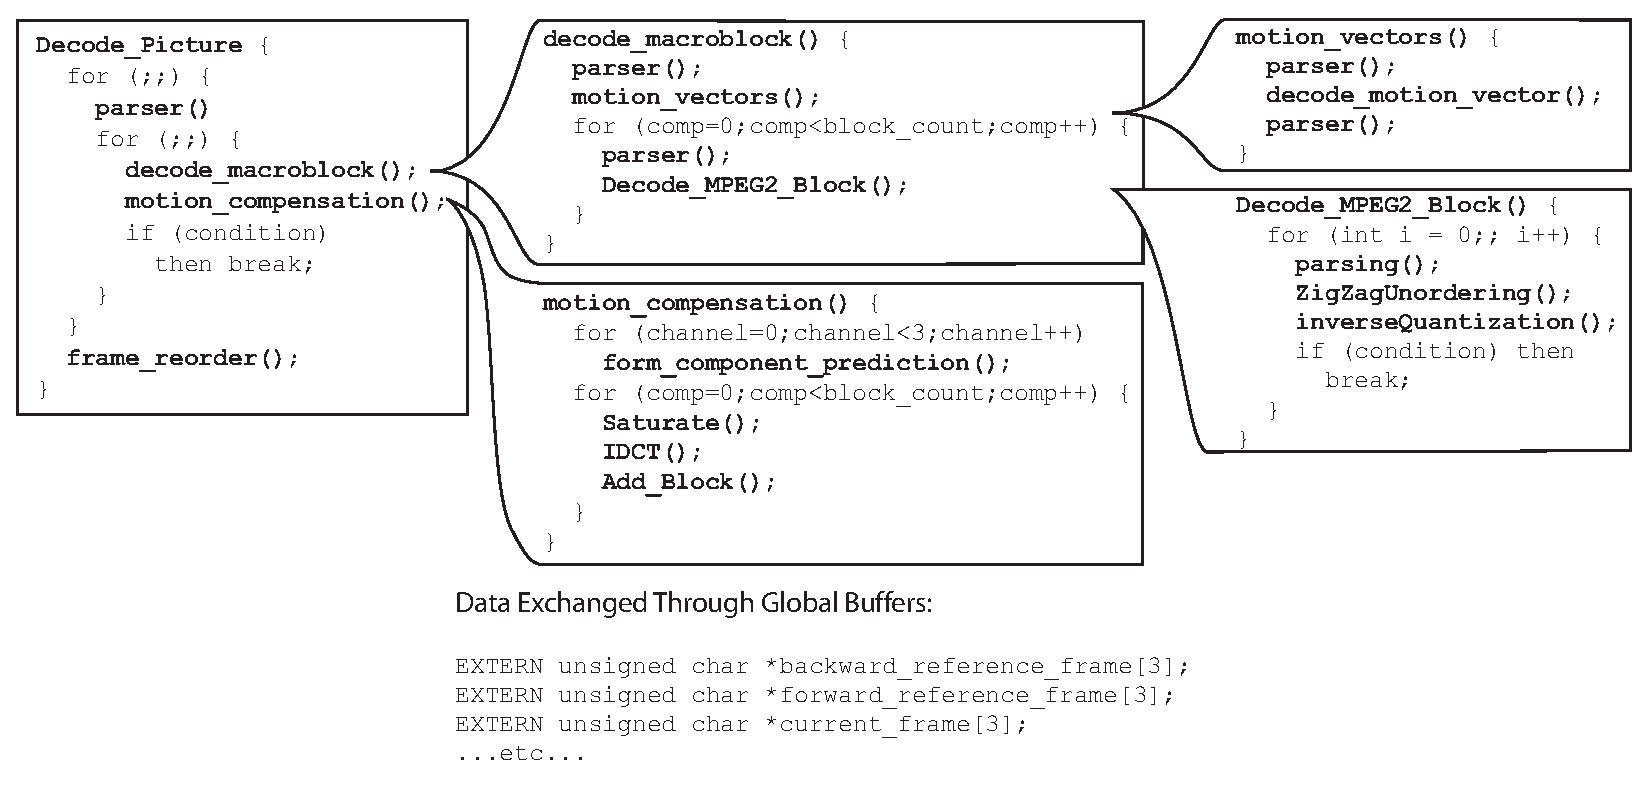
\includegraphics[scale=0.5, angle=0]{./call_diagram.eps}
    \caption{Simplified call-trace diagram for C decoder.}
    \label{fig:call-diagram}
  \end{center}
\end{figure}

\section{Usefulness of Teleport Messaging}
\label{sec:teleport_useful}

Teleport messaging is a useful language construct, as 
demonstrated by its importance in handling control messages 
in the decoder and encoder. 
Figures~\ref{table:enumerate_messages_decoder}~and~\ref{table:enumerate_messages_encoder} 
show the important control parameters that are sent by 
teleport messages in the MPEG-2 codecs. The number of 
subscribers for each message type highlights the usefulness 
of messages. 

\begin{figure}[h]
  \begin{center}
\begin{minipage}{\textwidth}
\renewcommand{\thempfootnote}{
  \arabic{footnote}
}
    \begin{tabular}{|p{1.7in}|l|l|p{0.9in}|p{0.9in}|}
\hline
\textbf{Message Content} & \textbf{Frequency} & \textbf{Regular} & \parbox{0.9in}{\textbf{Number of\\ Subscribers}} & \parbox{0.91in}{\vspace{0.04in} \textbf{Number of\\Subscriber\\Types} \vspace{0.04in}} \\
\hline
quantization scale code & macroblock & no & 2 & 2 \\
quantization tables & video & yes & 2 & 2 \\
macroblock type & macroblock & yes & 4 & 2 \\
picture type & picture & yes & 4 & 2 \\
motion vector resets & macroblock & no & 1 & 1 \\
\addtocounter{footnote}{1}
reference pictures & picture & no & many\footnote{One for every block in all color channels over a picture.} & 1 \\
\hline
    \end{tabular}
\end{minipage}
  \end{center}
  \caption{Important control parameters sent through the decoder using teleport messaging.}
  \label{table:enumerate_messages_decoder}
\end{figure}

\begin{figure}[h]
  \begin{center}
\begin{minipage}{\textwidth}
  \renewcommand{\thempfootnote}{
\arabic{footnote}
}
     \begin{tabular}{|p{1.7in}|l|l|p{0.9in}|p{0.9in}|}
\hline
\textbf{Message Content} & \textbf{Frequency} & \textbf{Regular} & \parbox{0.9in}{\textbf{Number of\\ Subscribers}} & \parbox{0.91in}{\vspace{0.04in} \textbf{Number of\\ Subscriber\\ Types} \vspace{0.04in}} \\
\hline
quantization scale code & macroblock & no & 2 & 2 \\
quantization tables & video & yes & 1 & 1 \\
macroblock type & macroblock & yes & 4 & 2 \\
picture type & picture & yes & 4 & 4 \\
\addtocounter{footnote}{1}
reference pictures & picture & no & many\footnote{Once for every macroblock in all color channels over a picture.} & 2 \\
\hline
    \end{tabular}
\end{minipage}
  \end{center}
  \caption{Important control parameters sent through the encoder using teleport messaging.}
  \label{table:enumerate_messages_encoder}
\end{figure}

Messaging's impact on programmability is evident by 
considering how the C code exposes control relevant information. 
The C code passes data and control parameters through function 
parameters and a global address space. Figure~\ref{fig:c-arrow-diagram} shows the functional
units in the C decoder\footnote{A functional unit might contain multiple functions with
similar or related behaviors.}, the input bitstream, output video, and the shared 
address space. Arrows represent communication dependencies between the blocks. 
While the C implementation is natural --- for C code --- it would be difficult for a 
programmer or compiler to extract 
parallelism\footnote{Because
the analysis of data access patterns is complicated and 
correctness verification for optimizations becomes impractical, 
a compiler will make a pessimistic decision.}.

\begin{figure}[h]
  \begin{center}
    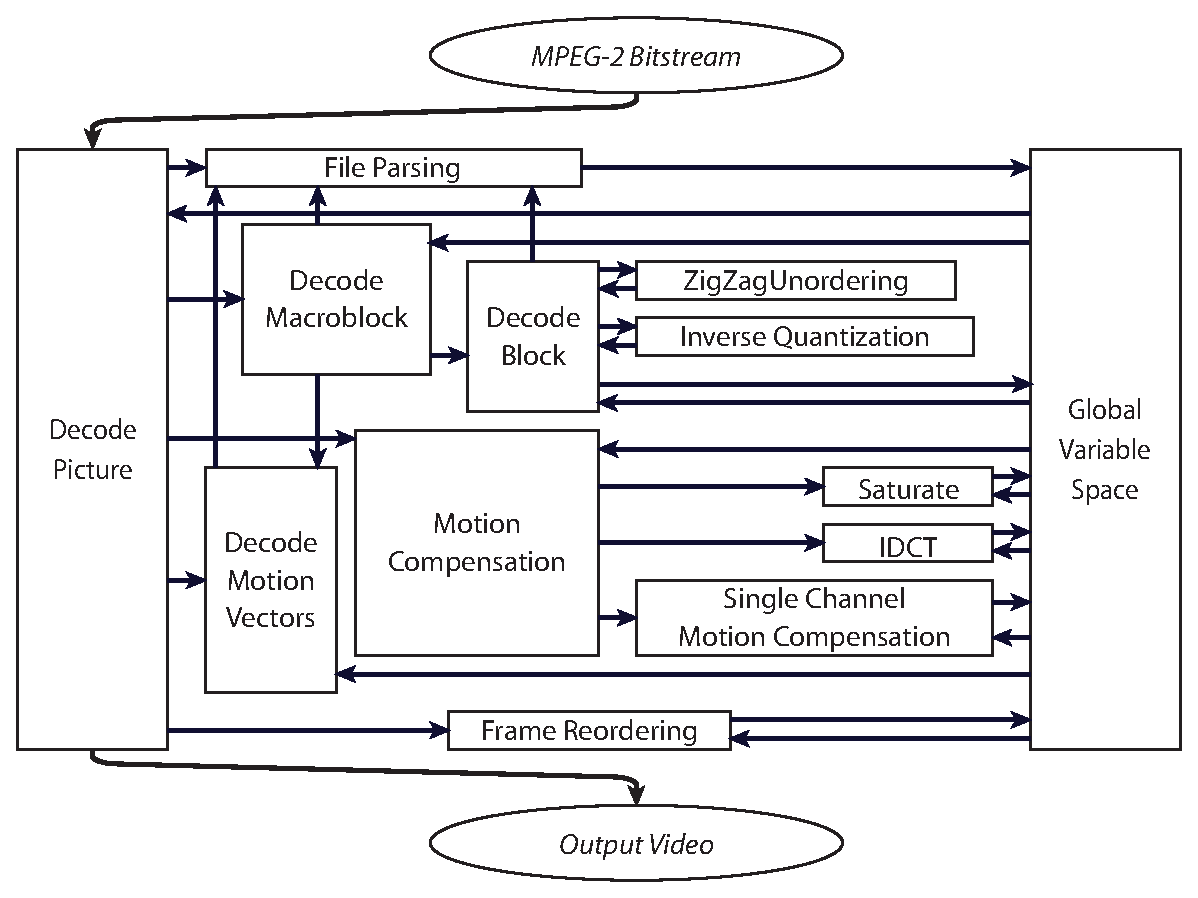
\includegraphics[scale=0.7, angle=0]{./functional_units.eps}
    \caption{Communication dependencies between functional units in the C code.}
    \label{fig:c-arrow-diagram}
  \end{center}
\end{figure}

Teleport messaging provides a point to point connection layer 
which a programmer can emulate in the dataflow layer by 
embedding control parameters in the data channels. While
StreamIt provides the feedback loop construct
to send information upstream, messaging is often more
appropriate for altering upstream state. 

Upstream reference frame passing in the encoder is used as an example. 
A feedback loop structure is impossible here, due to the fact that 
only some pictures should be sent upstream as reference pictures, 
and the information about which pictures to send upstream is not 
available at compile time. This would require the feedback loop to 
process messages regarding picture type and implement a dynamic 
rate splitter and joiner. This is not intuitive to implement, 
nor would it be easy for the compiler to analyze. Without B 
pictures the feedback loop structure needed to ensure that 
each motion estimation filter received the right reference frame 
immediately before the first block of a picture would still be 
non-trivial. Replacing the messaging scheme with a feedback loop 
would also effectively require the motion estimation filters to 
operate at a picture granularity, since each work execution 
would receive a reference picture, and this would limit 
parallelism by preventing estimation to be expressed at a block 
granularity. 

This chapter has given specific instances of where StreamIt improved
programmer productivity. Personal qualitative observations on the entire
implementation process are also pertinent. I found programming in StreamIt
to be very intuitive.
MPEG-2 decomposed naturally into concise independent filters. 
Filters make a program more modular than equivalent C code, 
which made it easy to change the encoder and decoder
stream graphs as my understanding of MPEG-2 improved. For the purposes
of correctness verification and performance comparisons it was much easier
to extract functional units from the StreamIt code than the C code.

